\documentclass[11pt,a4paper]{article}
\usepackage[T1]{fontenc}
\usepackage{lmodern}
\usepackage[margin=25mm]{geometry}
\usepackage{amsmath,booktabs,graphicx,tabularx}
\usepackage[hidelinks]{hyperref}
\usepackage{microtype}
\usepackage[font=small,labelfont=bf]{caption}
\graphicspath{{figures/}{analysis/outputs/flight1_2026-11-14/figures/}}
\setlength{\parskip}{0.35em}
\setlength{\parindent}{0pt}
\hypersetup{pdftitle={Paired Evaluation of Residual Soft Actor--Critic Control for Multirotor Flight},
  pdfauthor={UC San Diego Data Science Capstone Project}}
\title{Paired Evaluation of Residual Soft Actor--Critic Control for Multirotor Flight}
\author{UC San Diego Data Science Capstone Project}
\date{Statistical analysis: 14 November 2026\\Numerical review: 15 November 2026}

\begin{document}
\maketitle
\begin{abstract}
We assessed whether a trained residual Soft Actor--Critic (SAC) policy improved multirotor control relative to a fixed proportional--integral--derivative (PID) baseline. Our retrospective analysis comprised 420 Isaac Sim flight records, forming 210 controller pairs across seven scenarios, three wind profiles, and ten environment seeds per condition. We estimated paired differences in position root mean squared error (RMSE), constructed pointwise 95\% bootstrap intervals, and applied Holm-adjusted two-sided Wilcoxon signed-rank tests. SAC achieved lower recorded RMSE in all 180 open-air pairs. The equally weighted open-air mean flight-level RMSE decreased from 0.884\,m to 0.115\,m, an 87.0\% reduction; the mean paired difference was $-0.769$\,m (95\% seed-block interval: $-0.873$ to $-0.685$\,m). Twenty of the 21 primary condition comparisons rejected after adjustment. Both modes failed all strong-wind Dijkstra cases, with zero recorded SAC corrections consistent with launch-stage failure. Our findings support improved tracking for the evaluated checkpoint and baseline, subject to one training lineage, ten environment seeds, and unequal observed flight lengths.
\end{abstract}

\section{Objective and experimental scope}
We examined the magnitude, consistency, and uncertainty of residual SAC's contribution to PID flight control. The policy adds four learned thrust and torque corrections to the PID command before motor mixing. We analyzed the fixed \texttt{flight1/final\_model.zip} checkpoint, trained for 1,500,000 decisions with training seed 0. Its observation and action dimensions are 128 and four. The recorded evaluation, dated 4 November 2026, used a frozen deterministic policy and simulator ground-truth state\cite{source}.

Our benchmark comprised six open-air scenarios---hover, straight flight, turns/waypoints, altitude changes, circle, and figure eight---and one Dijkstra obstacle-navigation scenario with a planned route of 6.98\,m. The three wind profiles were training-range mean wind of 2--7\,m/s, stronger and faster unseen gusts, and outside-range mean wind of 8--10\,m/s. The outside-range label refers to this checkpoint's final-stage mean-wind training maximum of 7\,m/s. It does not bound instantaneous wind during gusts. Training calm-flight probabilities do not determine evaluation weights.

\section{Data integrity and statistical methods}
\subsection{Paired design and validation}
Our dataset contains seven scenarios $\times$ three wind profiles $\times$ ten seeds $\times$ two controllers, yielding 420 records and 210 pairs. Seeds 300000--300009 recur across conditions. We matched flights by scenario, wind profile, and environment seed, then verified agreement in recorded wind seed, mean wind speed when present, and reference-route duration.

We found no duplicate flights or missing pairs. Flight CSV records agreed with the archived JSON and recomputed source summaries. The evaluation documentation states that paired routes and initial conditions were shared. Exact reset vectors and reference hashes are absent from the summaries, limiting independent verification of those additional properties.

We independently audited all nine analytical tables against the original archived flight CSV. The audit enumerated exact-test sign assignments, calculated binomial probabilities, reconstructed BCa intervals with an explicit jackknife, and checked 12,370 fields. All comparisons passed within the specified numerical tolerances.

\subsection{Effects, uncertainty, and multiplicity}
For condition $c$ and seed $i$, our primary effect was
\begin{equation}
d_{c,i}=\mathrm{RMSE}_{\mathrm{PID+SAC},c,i}-\mathrm{RMSE}_{\mathrm{PID},c,i}.
\end{equation}
Negative values favor SAC. We report controller means, paired mean and median differences, paired-difference standard deviations, and win counts. Percentage reduction is calculated from controller means rather than by averaging seed-specific percentages.

We constructed pointwise 95\% bias-corrected and accelerated (BCa) intervals with 50,000 bootstrap resamples and deterministic resampling seeds\cite{bootstrap}. For each condition, we resampled complete paired differences. For overall benchmarks, we first averaged the selected fixed conditions within each environment seed and then resampled the ten resulting seed blocks. This preserves dependence associated with reused seeds. Overall results are means of flight-level RMSE, rather than RMSE calculated from concatenated time samples. Conditions receive equal weight within each benchmark.

Our primary tests were two-sided Wilcoxon signed-rank tests\cite{wilcoxon}, Holm-adjusted across 21 scenario--wind comparisons at $\alpha=0.05$\cite{holm}. The signed-rank null concerns a difference distribution symmetric about zero; it is not a direct test of equality of means. A separately Holm-adjusted exact sign-test family provided a direction-only robustness check\cite{binomial}. We interpreted both families without selecting the more favorable test. Confidence intervals remain pointwise, without simultaneous coverage across conditions.

Secondary continuous outcomes were cross-track RMSE, maximum position error, maximum cross-track error, and motor saturation fraction, with 84 comparisons in a separate Holm family. We analyzed completion, failure, and reported collision using exact McNemar tests with a separate 21-test family per outcome\cite{mcnemar}. Controller-rate intervals were exact binomial intervals, not intervals for paired rate differences. These families do not imply one global 5\% error rate across all reported analyses.

\subsection{Terminated flights and sensitivity analysis}
We retained failed flights in primary analyses. Their recorded errors describe the portions actually flown. We examined decision-count differences and defined a separate sensitivity subset requiring both flights to be nonfailed and to have equal recorded counts. This subset conditions on survival and may introduce selection bias. Equal counts alone do not establish identical sample times.

\section{Results}
\subsection{Open-air tracking}
SAC achieved lower recorded position RMSE in all 180 open-air pairs. Table~\ref{tab:open} summarizes the three wind profiles. Across the equally weighted open-air benchmark, mean flight-level RMSE decreased from 0.884\,m to 0.115\,m. The mean paired difference was $-0.769$\,m, with a pointwise 95\% seed-block interval of $[-0.873,-0.685]$\,m, corresponding to an 87.0\% reduction.

\begin{table}[htbp]
\centering\small
\begin{tabular}{lrrrr}
\toprule
Wind profile & Pairs & PID (m) & PID+SAC (m) & Reduction \\
\midrule
Training range & 60 & 0.502 & 0.082 & 83.6\% \\
Unseen gusts & 60 & 0.497 & 0.082 & 83.5\% \\
Outside range & 60 & 1.653 & 0.181 & 89.0\% \\
\bottomrule
\end{tabular}
\caption{Open-air mean flight-level position RMSE. All 60 pairs favored SAC within each profile. Reductions use unrounded controller means.}
\label{tab:open}
\end{table}

SAC's absolute error increased under outside-range wind, although its relative advantage over PID remained large. Similar training-range and unseen-gust averages do not establish equivalence. Figure~\ref{fig:overview} shows benchmark uncertainty with repeated seed dependence preserved.

\begin{figure}[htbp]
\centering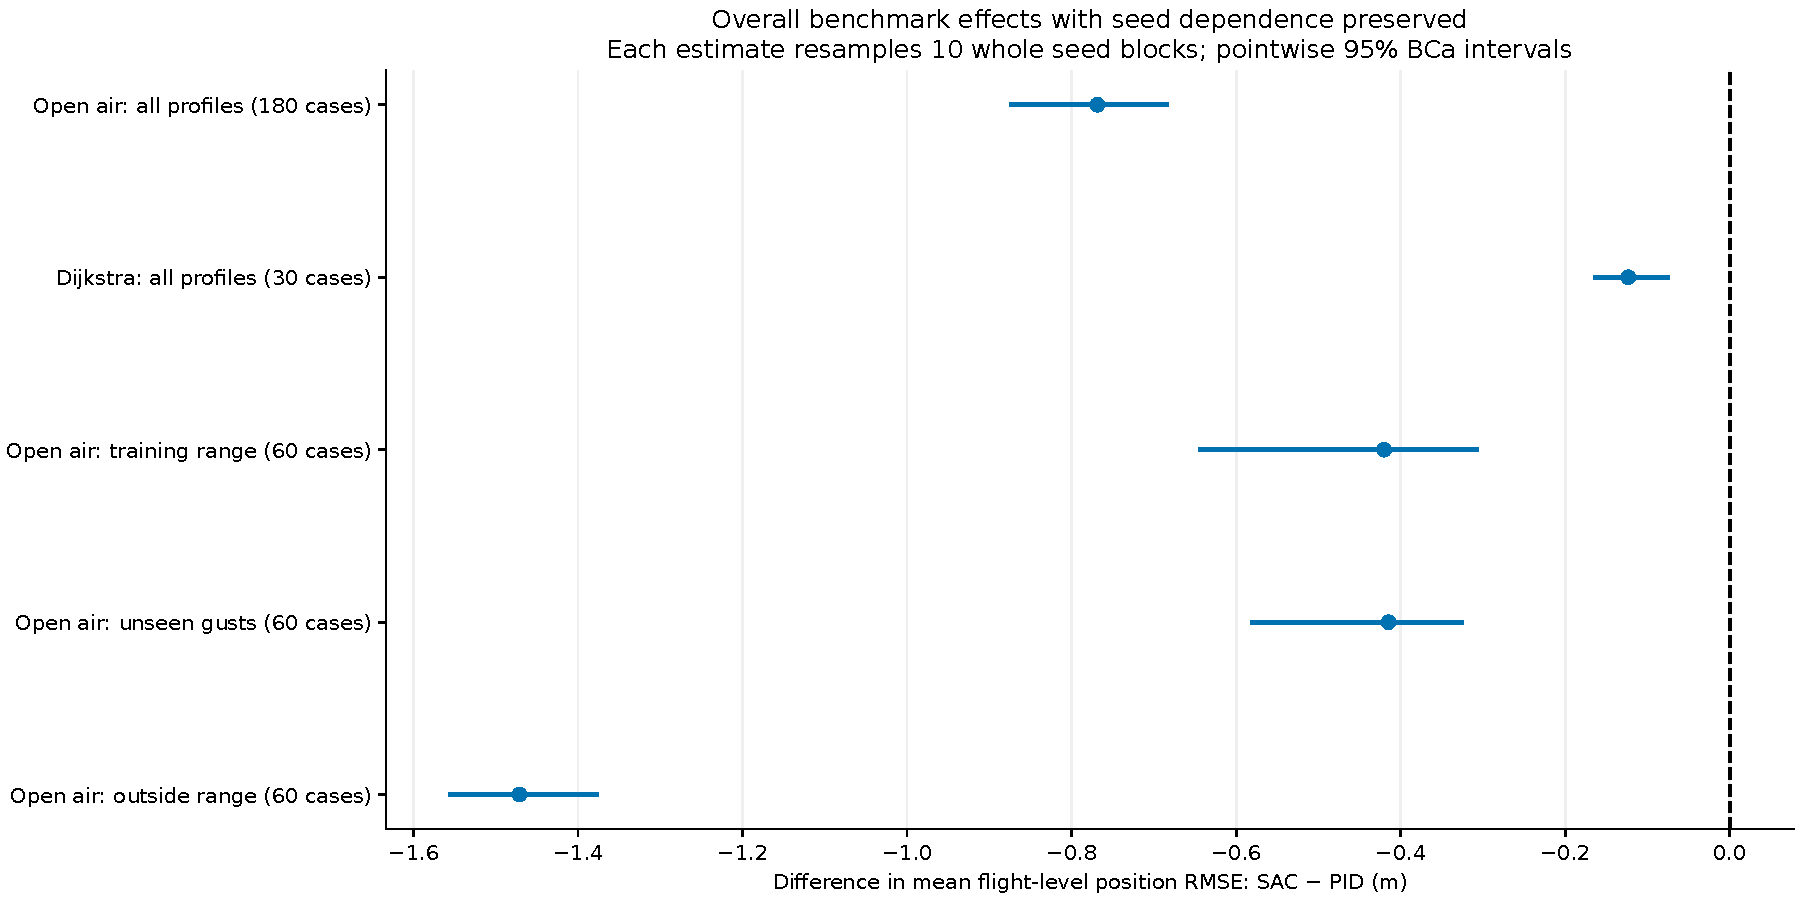
\includegraphics[width=\linewidth]{seed_cluster_overview.pdf}
\caption{Fixed-benchmark mean paired effects. Pointwise 95\% BCa intervals resample ten whole environment-seed blocks.}
\label{fig:overview}
\end{figure}

\subsection{Condition-specific inference}
Twenty of the 21 mean differences favored SAC. The corresponding primary signed-rank tests rejected after Holm adjustment, with adjusted $p=0.04102$. Separately adjusted sign tests also rejected in those 20 conditions. Strong-wind Dijkstra was the sole exception. Complete primary estimates are provided in Appendix~\ref{app:primary}; Figure~\ref{fig:conditions} displays the paired effects.

\begin{figure}[htbp]
\centering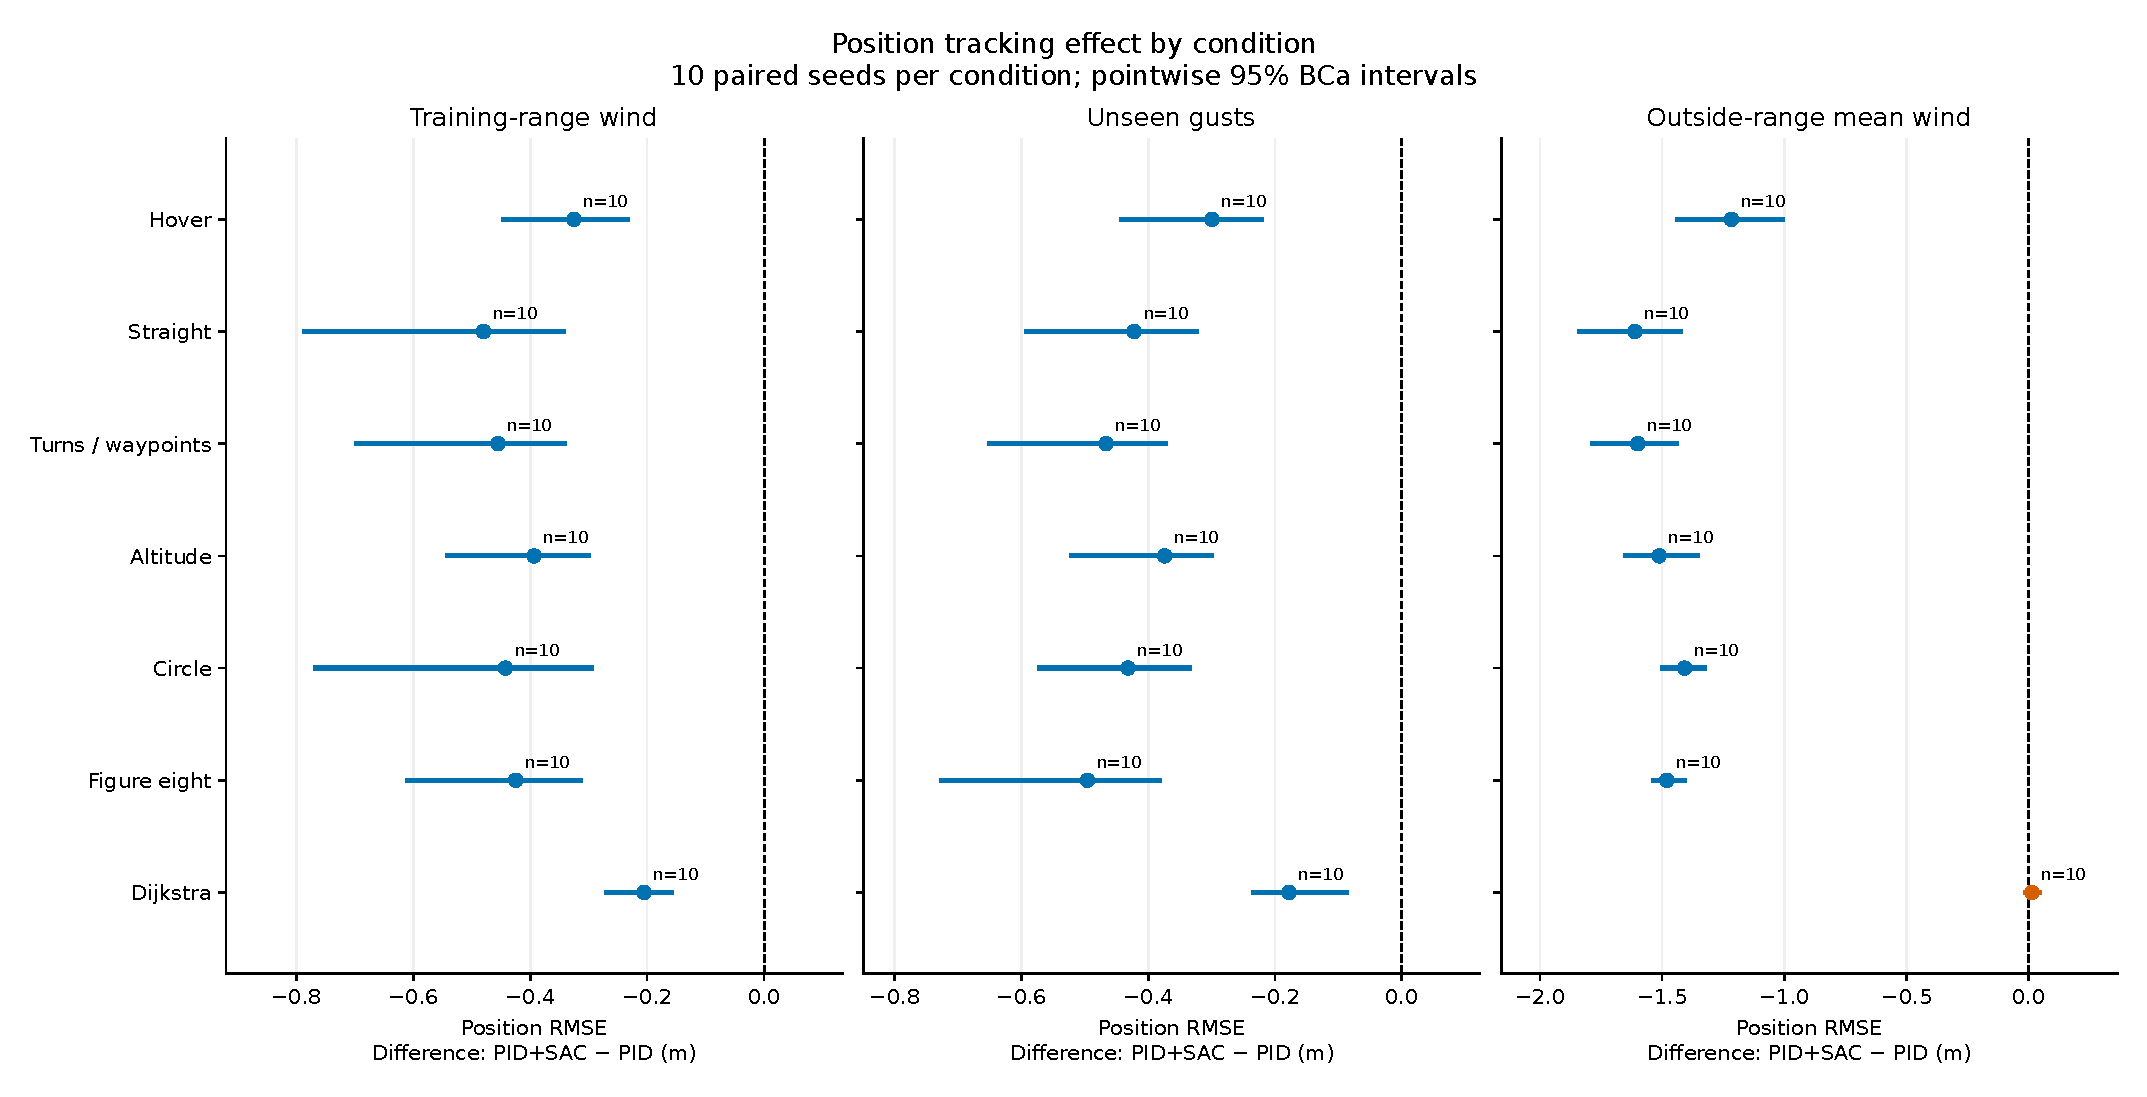
\includegraphics[width=\linewidth]{rmse_effects.pdf}
\caption{Condition-specific mean RMSE differences. Negative values favor SAC. Confidence intervals are pointwise and are distinct from the Holm-adjusted hypothesis tests.}
\label{fig:conditions}
\end{figure}

\subsection{Navigation and completion}
We observed improved Dijkstra tracking and completion in training-range wind and unseen gusts (Table~\ref{tab:nav}). Both modes failed all ten outside-range navigation cases. In that condition, the mean RMSE difference was $+0.013$\,m (pointwise 95\% interval $[-0.015,+0.043]$\,m; adjusted $p=0.42578$). We did not detect a reliable difference, which does not establish equivalence.

\begin{table}[htbp]
\centering\small
\begin{tabular}{lrrrr}
\toprule
& \multicolumn{2}{c}{Mean RMSE (m)} & \multicolumn{2}{c}{Completed} \\
\cmidrule(lr){2-3}\cmidrule(lr){4-5}
Wind profile & PID & PID+SAC & PID & PID+SAC \\
\midrule
Training range & 0.391 & 0.186 & 2/10 & 9/10 \\
Unseen gusts & 0.399 & 0.221 & 0/10 & 7/10 \\
Outside range & 0.431 & 0.444 & 0/10 & 0/10 \\
\bottomrule
\end{tabular}
\caption{Dijkstra obstacle-navigation results. Error metrics summarize observed portions of flights, including terminated cases.}
\label{tab:nav}
\end{table}

All 14 failed PID+SAC flights had zero recorded mean residual magnitude. The evaluation documentation describes a departure of approximately 2.8\,s with the residual disabled. These observations are consistent with launch-stage failure. They characterize the complete navigation system but do not isolate the performance of an engaged airborne policy during those failed cases.

Across all cases, recorded completion counts were 8/210 for PID and 190/210 for PID+SAC; failure counts were 57/210 and 14/210; reported collision counts were 5/210 and 0/210. These pooled counts are descriptive. Within open-air scenarios, PID completed 6/180 and failed 37/180, whereas PID+SAC completed 174/180 and failed 0/180. All 37 PID open-air failures occurred under outside-range wind. A flight without failure did not necessarily satisfy the completion criterion.

Eight condition-specific completion comparisons rejected after adjustment of exact McNemar tests. No individual failure or collision comparison rejected within its adjusted family. Collision flags reflect the source workflow's geometric checks or proxies rather than an independently revalidated contact measurement.

\subsection{Observation length and secondary measurements}
Decision counts differed in 54/210 pairs. Early termination changes exposure duration and the route segments contributing to RMSE. The saved summaries do not permit common-time-window reconstruction. Our sensitivity subset retained 152 nonfailed, equal-count pairs across 20 conditions. Every represented mean difference favored SAC; 13 signed-rank comparisons rejected after the separate sensitivity-family adjustment. Strong-wind Dijkstra had no eligible pairs. This conditional result remains subject to survivor selection.

None of the 84 secondary continuous signed-rank comparisons rejected after Holm adjustment. With ten nonzero pairs, the minimum two-sided exact $p$-value is $2/2^{10}=0.001953125$, exceeding the first Holm threshold $0.05/84\approx0.000595$. Accordingly, no rejection is attainable in that family at the current sample size under these exact tests. This does not establish absence of an effect.

Recorded motor saturation was zero in all flights. Mean normalized SAC residual magnitude increased from 1.039 in training-range open-air wind to 1.324 in outside-range wind. These measurements describe action magnitude and clipping, not physical energy, correction direction, wind alignment, or operational safety.

\section{Discussion and limitations}
Our findings indicate a substantial and consistent improvement in recorded open-air tracking for the evaluated residual policy and PID configuration. They also identify launch reliability as a separate navigation requirement. Aggregate RMSE alone cannot establish mission reliability, particularly when failures shorten observation horizons.

Our inference concerns environment-seed variation for one trained policy, not variation across independent training runs. The baseline gains, acceleration limits, and residual authority define the comparison; superiority over other PID tunings or disturbance-rejection controllers has not been established. Ground-truth state evaluation does not assess sensor-estimation noise, latency, or physical flight. Small binary-outcome samples further limit precision.

The saved summaries lack per-step reference, state, wind, correction, integral, and event traces needed for error-over-time curves, recovery after disturbances, directional wind classification, or correction--integral alignment. Final-goal completion time is not post-event recovery time. Our analysis is retrospective. Confirmation should use declared endpoints and evaluation cases held out from tuning and model selection.

\section{Conclusion}
We found that residual SAC substantially reduced recorded open-air position-tracking error relative to the specified PID baseline. Mean flight-level RMSE decreased by 87.0\% across the equally weighted open-air benchmark, and 20 of 21 primary condition comparisons rejected after multiplicity adjustment. Strong-wind obstacle navigation remained unsuccessful during the residual-disabled launch phase. The results support the evaluated policy's tracking contribution while identifying takeoff reliability and broader validation as distinct requirements.

\section*{Data and analytical materials}
The accompanying nine CSV tables contain paired records, primary and secondary effects, outcomes, seed-block summaries, observation-length diagnostics, and control-effort measurements. We retain original evaluation files and configuration evidence with input, code, and artifact checksums to support traceability and reproducibility. Full inference details are documented in the accompanying statistical methods file.

\begin{thebibliography}{9}
\bibitem{source} UC San Diego Data Science Capstone Project. \emph{Flight SAC evaluation report and associated flight records}. Evaluation dated 4 November 2026; archived with the first flight SAC checkpoint.
\bibitem{bootstrap} SciPy. \emph{scipy.stats.bootstrap: Bootstrap confidence intervals}. \href{https://docs.scipy.org/doc/scipy/reference/generated/scipy.stats.bootstrap.html}{Official documentation}.
\bibitem{wilcoxon} SciPy. \emph{scipy.stats.wilcoxon: Paired signed-rank inference}. \href{https://docs.scipy.org/doc/scipy/reference/generated/scipy.stats.wilcoxon.html}{Official documentation}.
\bibitem{binomial} SciPy. \emph{scipy.stats.binomtest: Exact binomial inference}. \href{https://docs.scipy.org/doc/scipy/reference/generated/scipy.stats.binomtest.html}{Official documentation}.
\bibitem{mcnemar} statsmodels. \emph{Exact McNemar test}. \href{https://www.statsmodels.org/stable/generated/statsmodels.stats.contingency_tables.mcnemar.html}{Official documentation}.
\bibitem{holm} statsmodels. \emph{Multiple-testing procedures}. \href{https://www.statsmodels.org/stable/generated/statsmodels.stats.multitest.multipletests.html}{Official documentation}.
\end{thebibliography}

\clearpage
\appendix
\section{Complete primary condition estimates}\label{app:primary}
We report mean position RMSE, the SAC-minus-PID mean difference, pointwise 95\% BCa intervals, SAC win counts, and primary-family Holm-adjusted signed-rank $p$-values. Each row contains ten pairs. Intervals are not multiplicity-adjusted.

\begin{table}[htbp]
\centering
\resizebox{\linewidth}{!}{%
\begin{tabular}{llrrrrrr}
\toprule
Scenario & Wind & PID (m) & PID+SAC (m) & Difference (m) & 95\% CI (m) & SAC wins & Holm $p$ \\
\midrule
Hover & Training & 0.413 & 0.088 & $-0.325$ & $[-0.446,-0.234]$ & 10/10 & 0.04102 \\
Hover & Gusts & 0.387 & 0.088 & $-0.299$ & $[-0.442,-0.221]$ & 10/10 & 0.04102 \\
Hover & Outside & 1.432 & 0.216 & $-1.216$ & $[-1.437,-1.006]$ & 10/10 & 0.04102 \\
Straight & Training & 0.563 & 0.083 & $-0.480$ & $[-0.786,-0.343]$ & 10/10 & 0.04102 \\
Straight & Gusts & 0.505 & 0.083 & $-0.422$ & $[-0.592,-0.324]$ & 10/10 & 0.04102 \\
Straight & Outside & 1.784 & 0.173 & $-1.611$ & $[-1.838,-1.427]$ & 10/10 & 0.04102 \\
Turns & Training & 0.541 & 0.086 & $-0.455$ & $[-0.697,-0.342]$ & 10/10 & 0.04102 \\
Turns & Gusts & 0.551 & 0.085 & $-0.466$ & $[-0.650,-0.373]$ & 10/10 & 0.04102 \\
Turns & Outside & 1.791 & 0.192 & $-1.600$ & $[-1.783,-1.440]$ & 10/10 & 0.04102 \\
Altitude & Training & 0.488 & 0.095 & $-0.393$ & $[-0.541,-0.301]$ & 10/10 & 0.04102 \\
Altitude & Gusts & 0.467 & 0.093 & $-0.374$ & $[-0.520,-0.300]$ & 10/10 & 0.04102 \\
Altitude & Outside & 1.705 & 0.193 & $-1.512$ & $[-1.647,-1.357]$ & 10/10 & 0.04102 \\
Circle & Training & 0.514 & 0.072 & $-0.442$ & $[-0.768,-0.295]$ & 10/10 & 0.04102 \\
Circle & Gusts & 0.504 & 0.072 & $-0.432$ & $[-0.572,-0.335]$ & 10/10 & 0.04102 \\
Circle & Outside & 1.569 & 0.161 & $-1.408$ & $[-1.499,-1.327]$ & 10/10 & 0.04102 \\
Figure eight & Training & 0.495 & 0.070 & $-0.425$ & $[-0.609,-0.313]$ & 10/10 & 0.04102 \\
Figure eight & Gusts & 0.567 & 0.071 & $-0.496$ & $[-0.726,-0.382]$ & 10/10 & 0.04102 \\
Figure eight & Outside & 1.634 & 0.153 & $-1.481$ & $[-1.533,-1.410]$ & 10/10 & 0.04102 \\
Dijkstra & Training & 0.391 & 0.186 & $-0.205$ & $[-0.270,-0.159]$ & 10/10 & 0.04102 \\
Dijkstra & Gusts & 0.399 & 0.221 & $-0.178$ & $[-0.234,-0.087]$ & 9/10 & 0.04102 \\
Dijkstra & Outside & 0.431 & 0.444 & $+0.013$ & $[-0.015,+0.043]$ & 3/10 & 0.42578 \\
\bottomrule
\end{tabular}}
\caption{All primary condition-specific estimates. Wind labels abbreviate training range, unseen gusts, and outside range.}
\end{table}

\clearpage
\section{Supplementary figures}
\begin{figure}[htbp]
\centering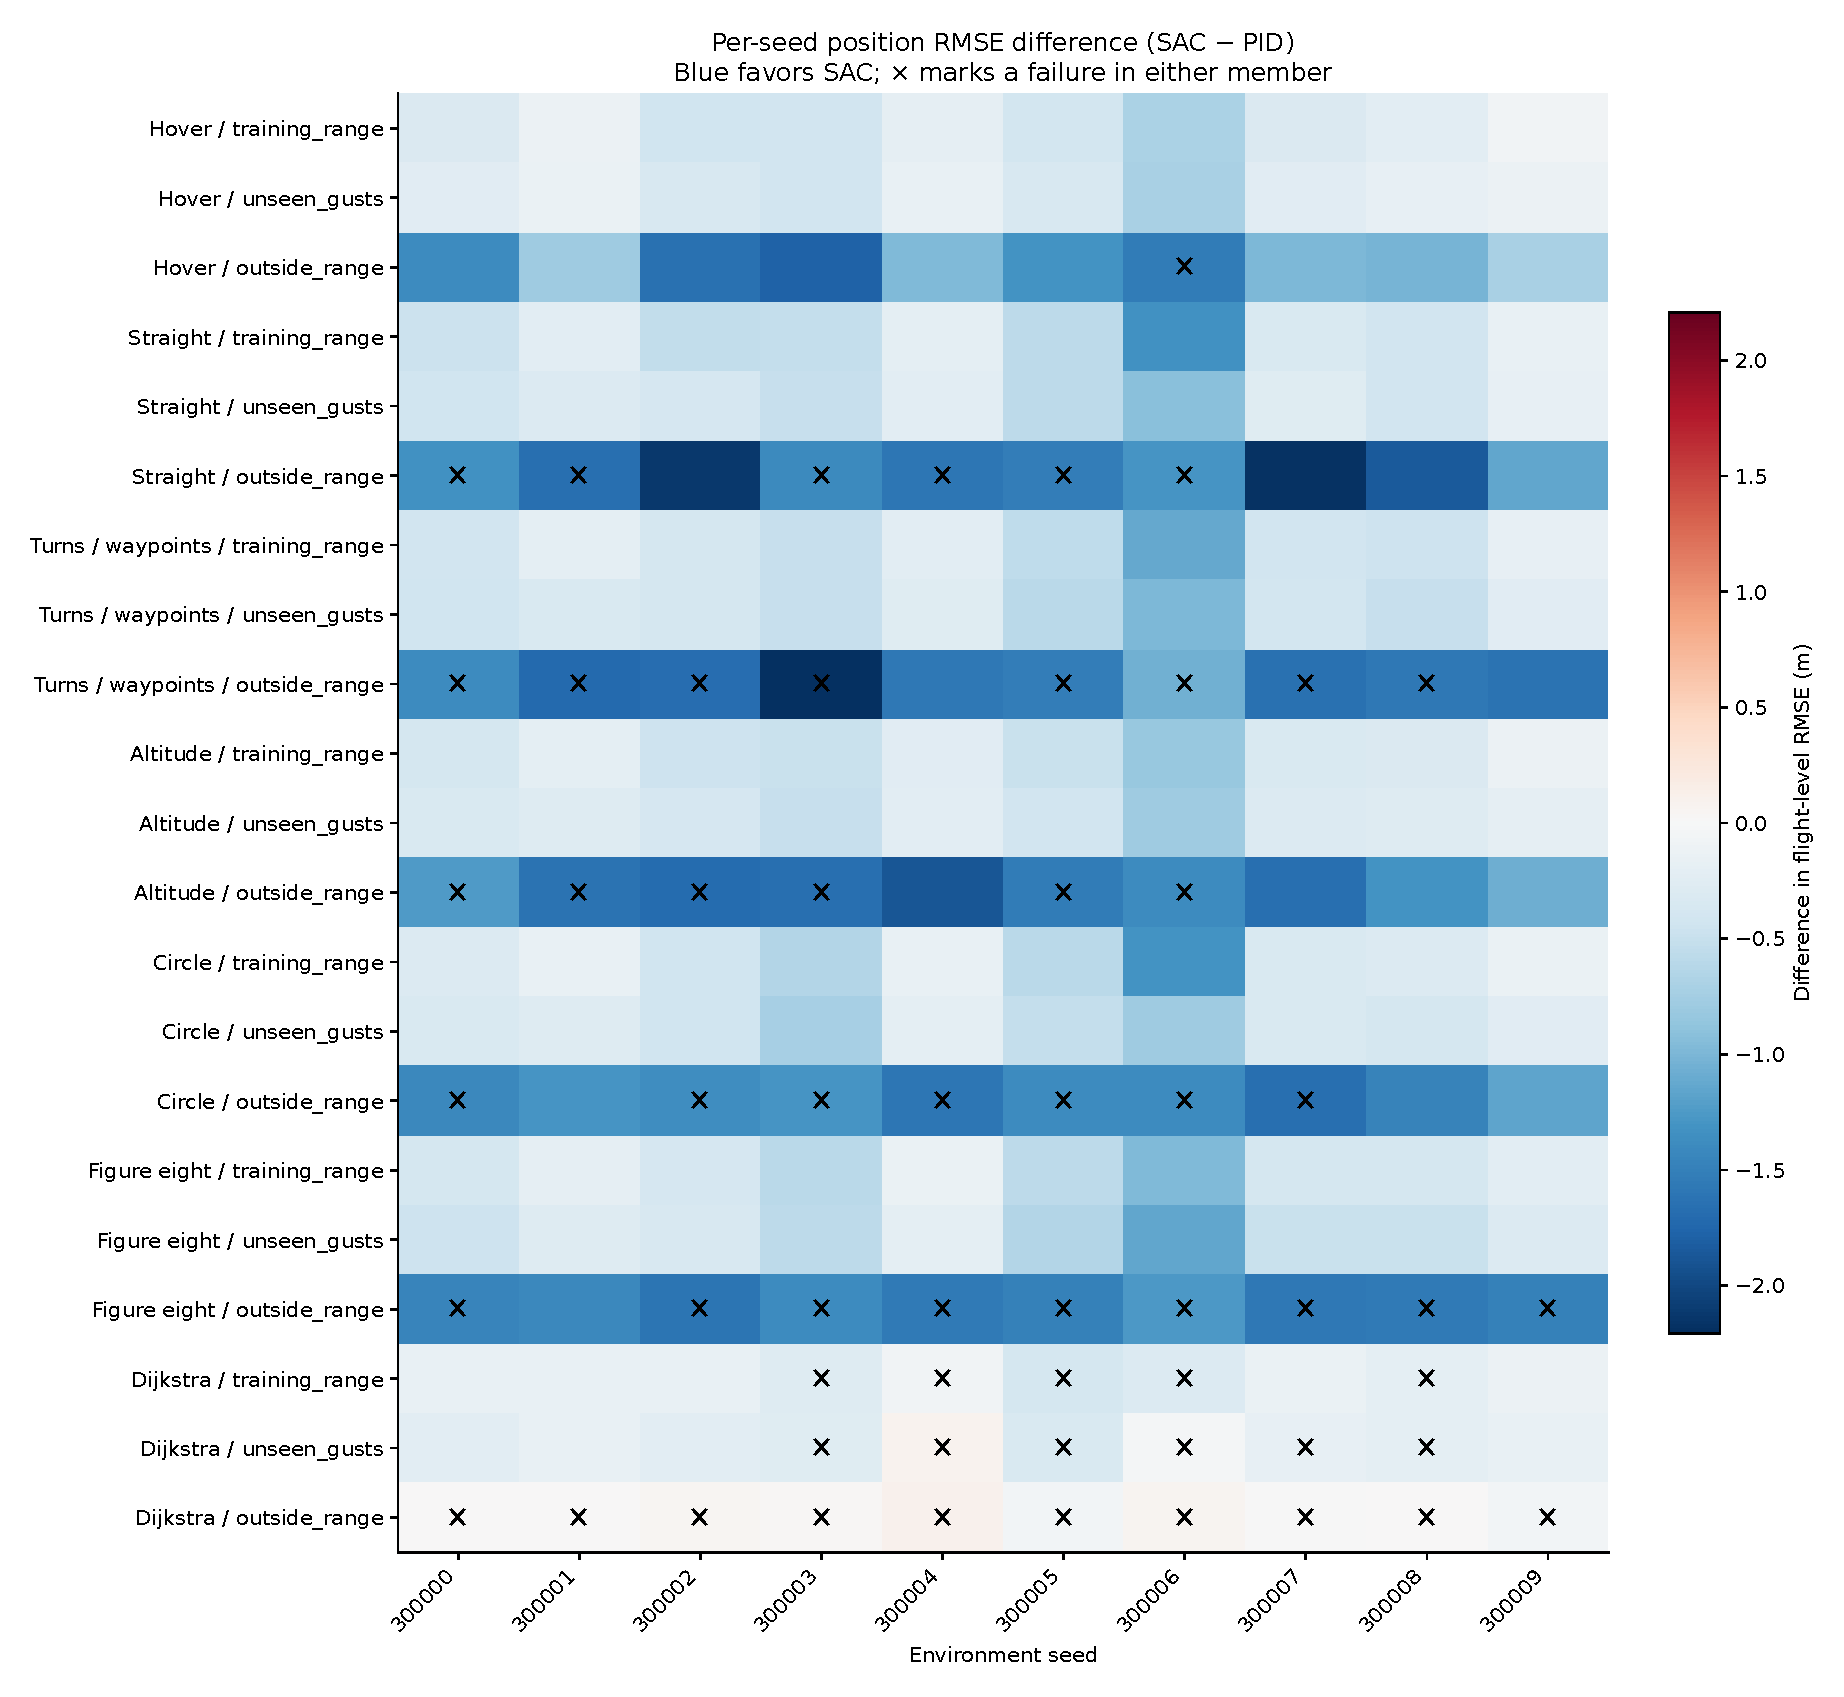
\includegraphics[width=.88\linewidth,height=.60\textheight,keepaspectratio]{seed_differences.pdf}
\caption{Individual paired differences by environment seed. Blue favors SAC; crosses mark a failure in either member. Reused seed identifiers remain grouped in overall inference.}
\end{figure}
\begin{figure}[htbp]
\centering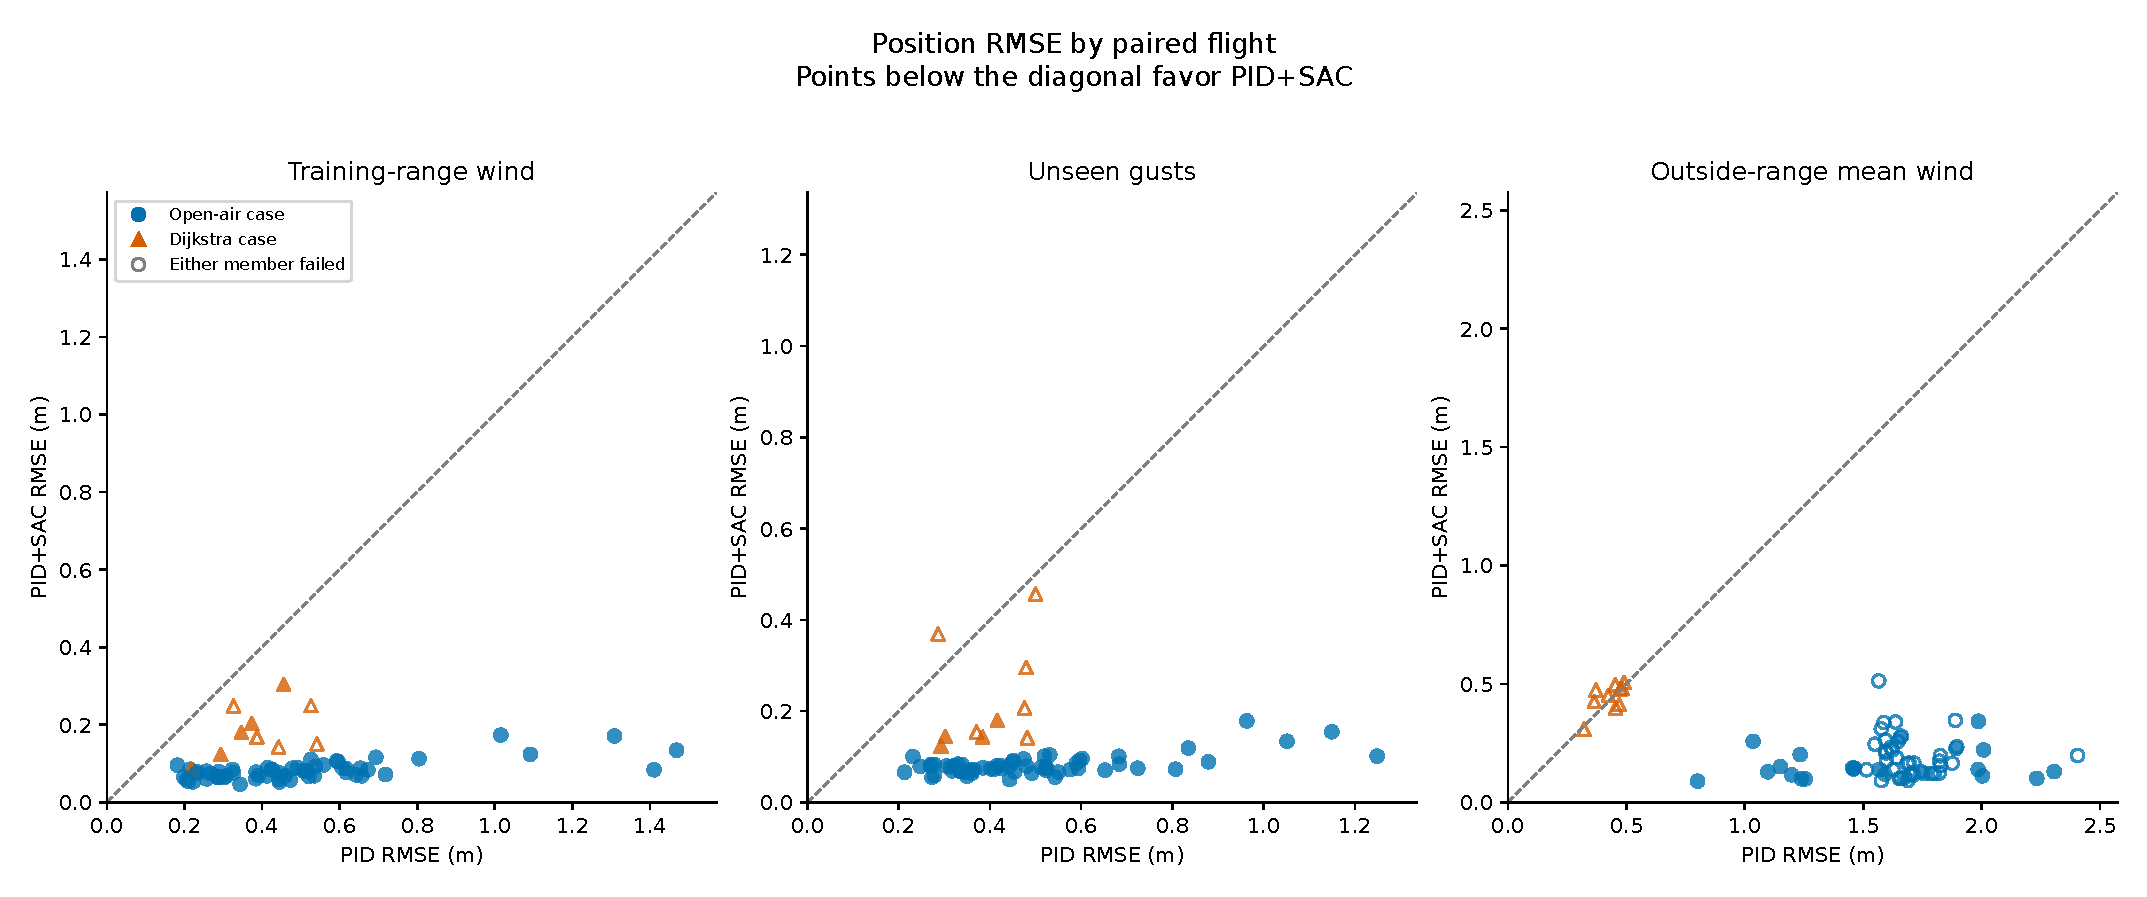
\includegraphics[width=\linewidth]{paired_scatter.pdf}
\caption{Individual controller comparisons. Points below the diagonal favor SAC; hollow markers denote a failure in either paired flight.}
\end{figure}
\clearpage
\begin{figure}[htbp]
\centering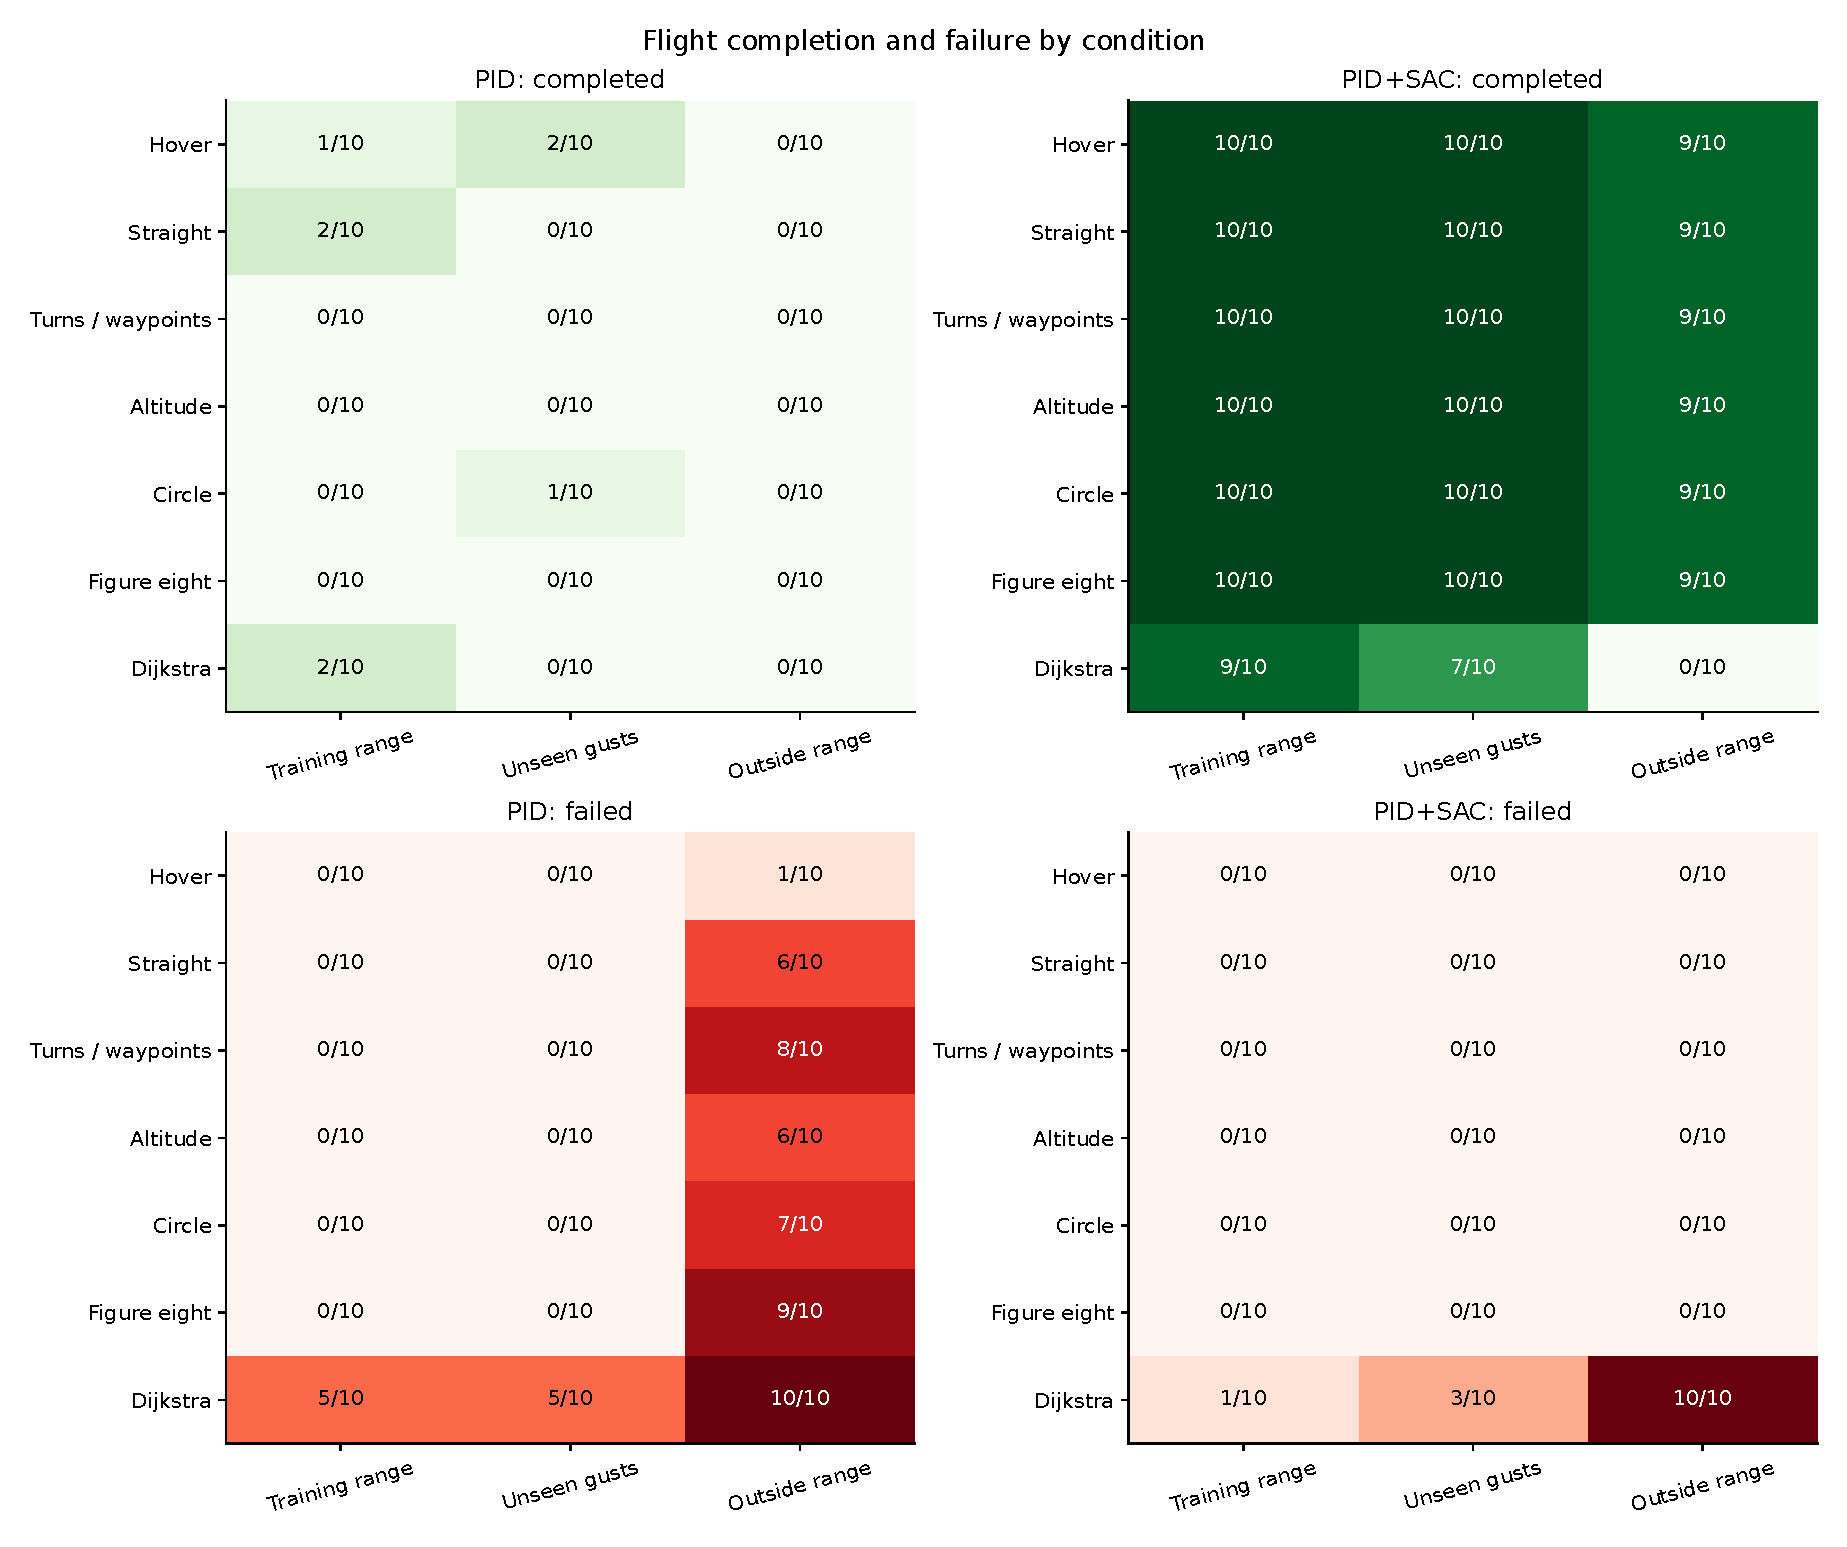
\includegraphics[width=.90\linewidth,height=.61\textheight,keepaspectratio]{outcomes.pdf}
\caption{Completion and failure counts. Absence of recorded failure does not necessarily satisfy the completion criterion.}
\end{figure}
\begin{figure}[htbp]
\centering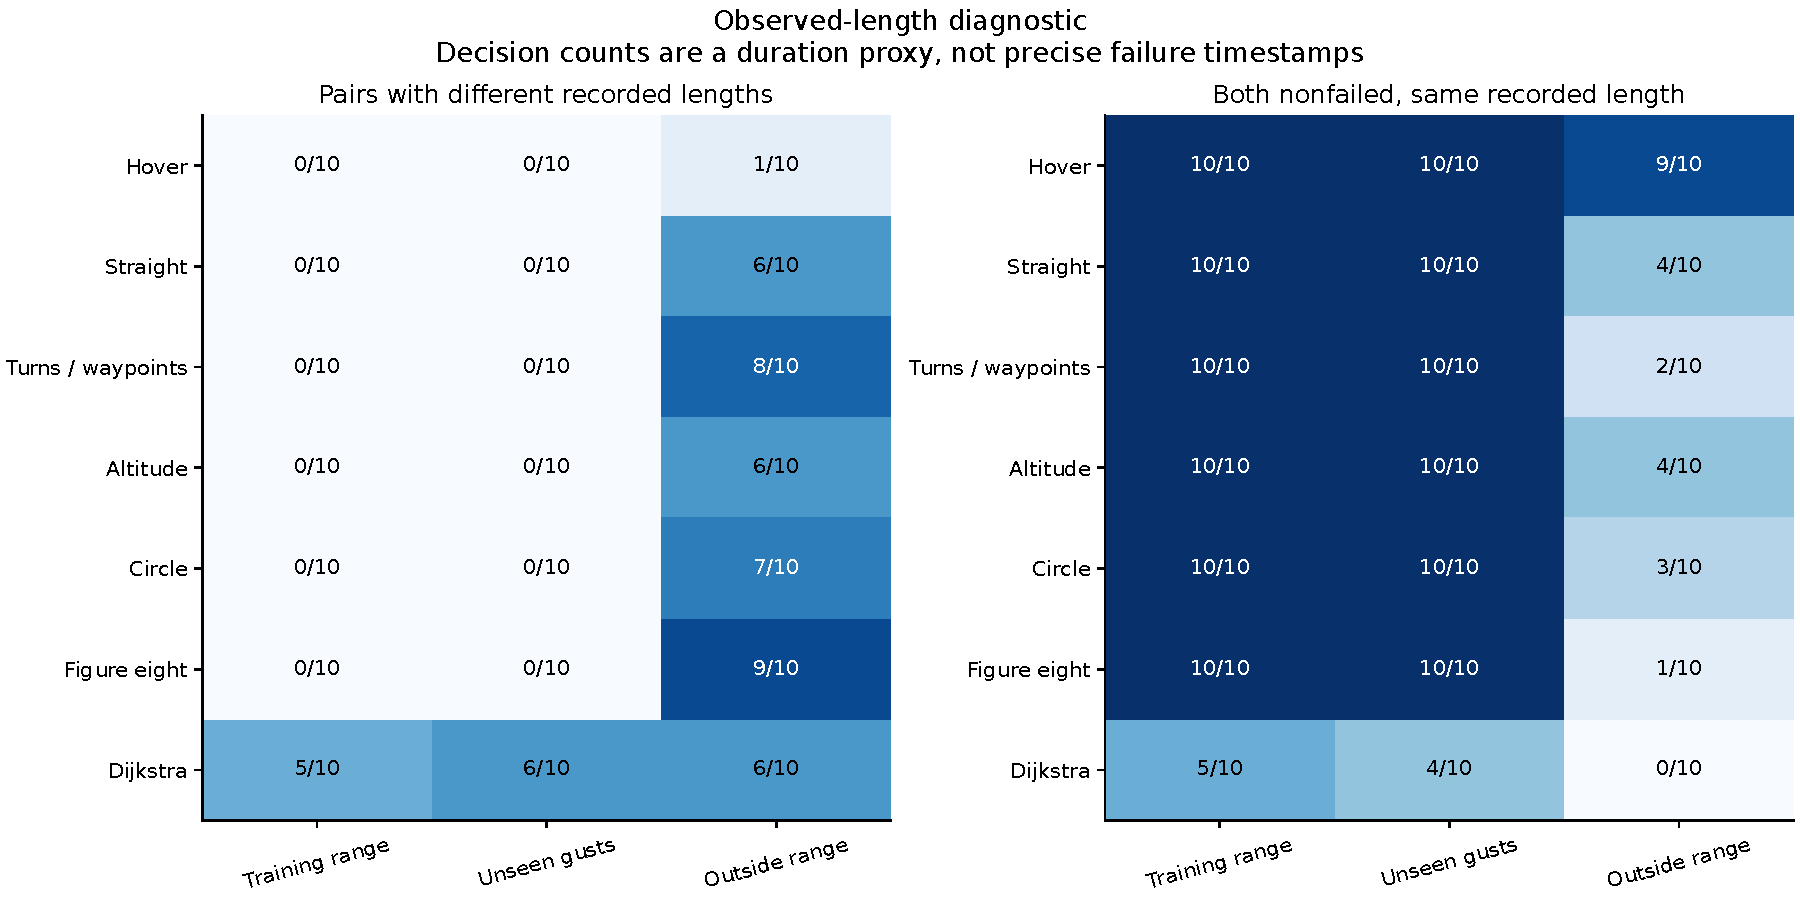
\includegraphics[width=\linewidth]{observed_lengths.pdf}
\caption{Observation-length diagnostics. The left panel shows unequal decision counts; the right shows nonfailed, equal-count pairs eligible for sensitivity analysis.}
\end{figure}
\clearpage
\begin{figure}[htbp]
\centering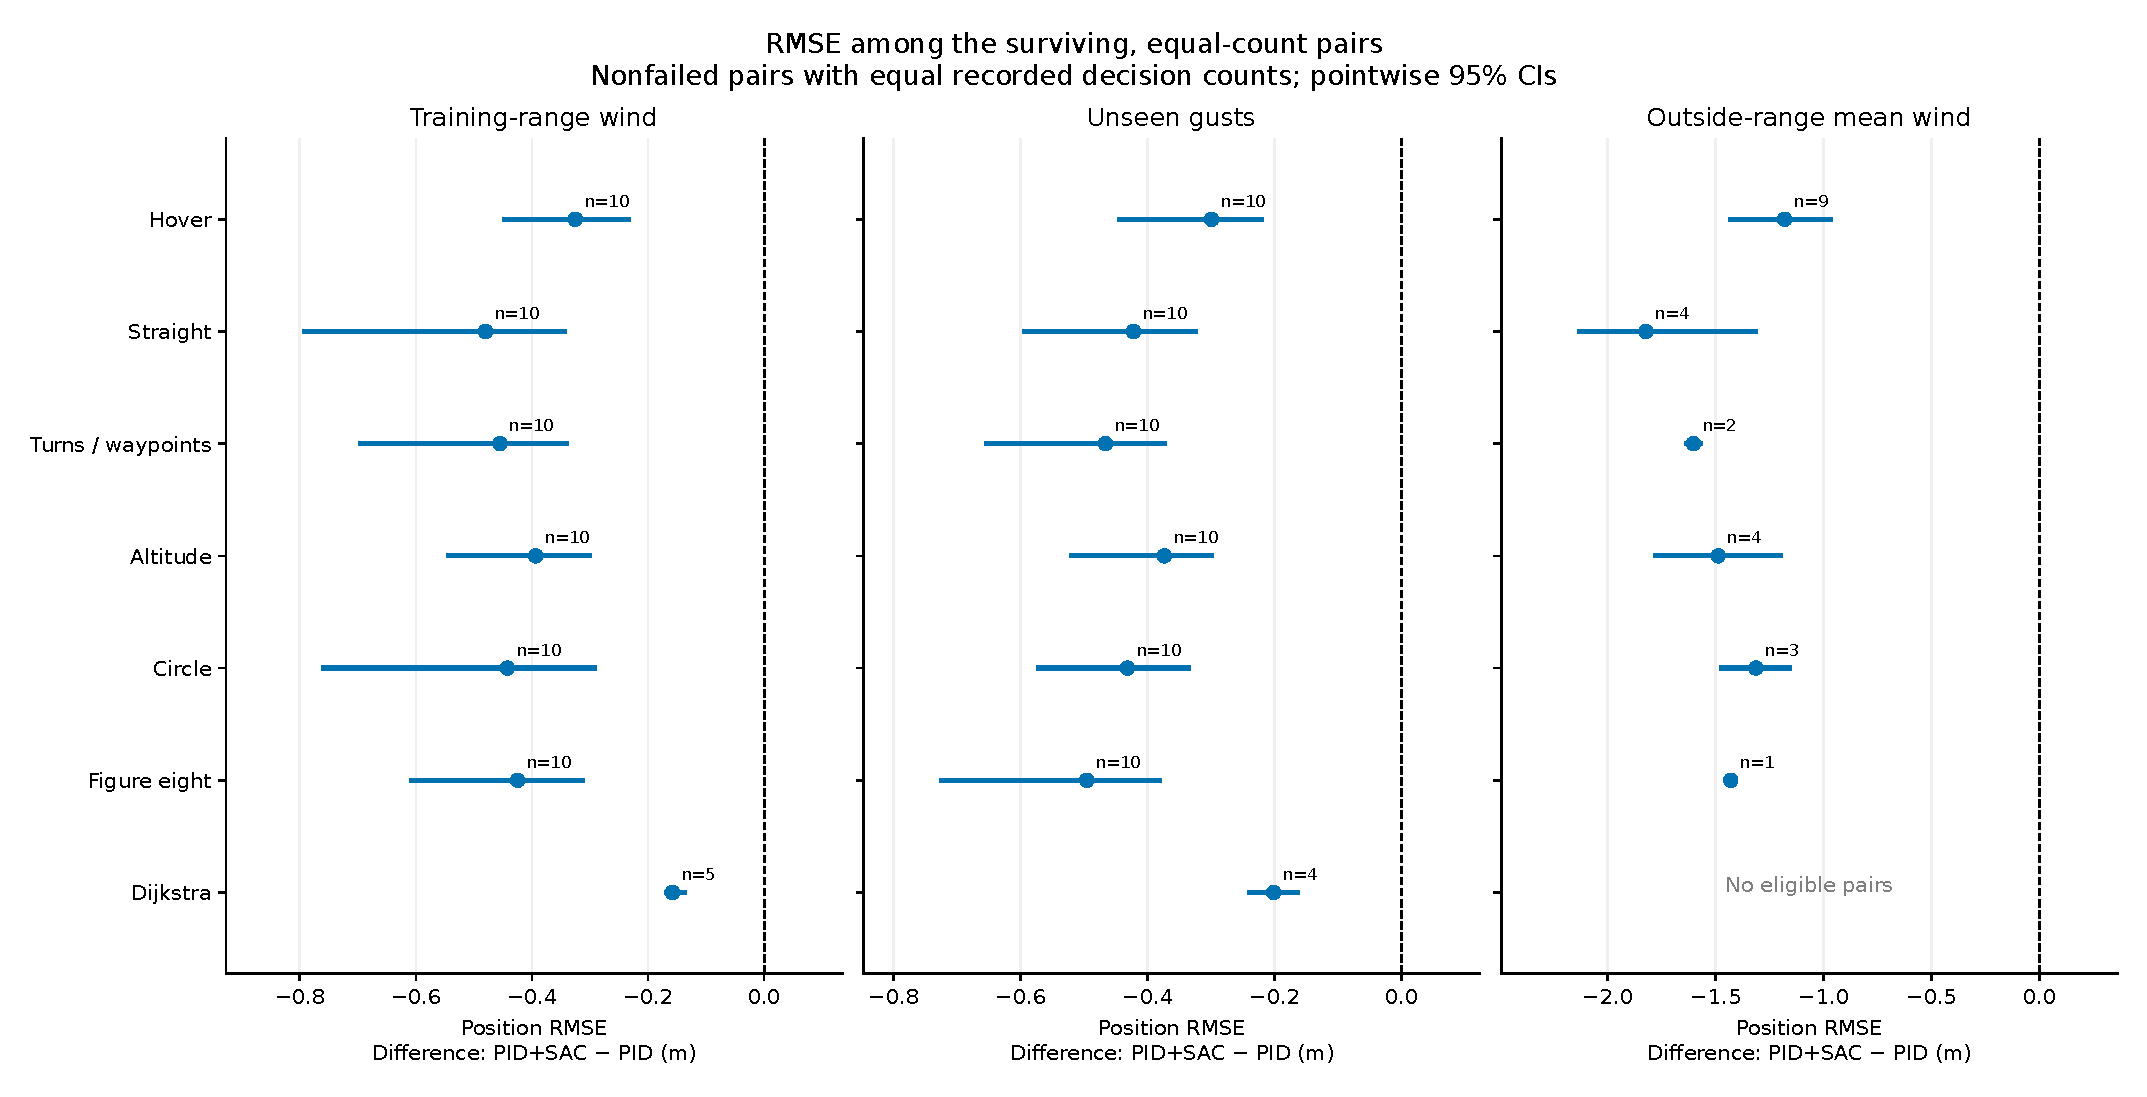
\includegraphics[width=\linewidth]{rmse_sensitivity.pdf}
\caption{Survivor-conditioned sensitivity estimates. All represented means favor SAC, but subgroup sizes are small and selection can bias comparisons. Strong-wind Dijkstra has no eligible pairs.}
\end{figure}
\end{document}
